\documentclass[10pt,ngerman]{beamer}

\usepackage[ngerman]{babel}

\usetheme[progressbar=frametitle]{metropolis}
\usepackage{appendixnumberbeamer}

\usepackage[utf8]{inputenc}

\usepackage{csquotes}

\usepackage[bibencoding=utf8,
			sortlocale=de,
			style=numeric,
			pagetracker=true,
			autocite=inline,
			backrefstyle=three+,
			date=short,
			sorting=nty,
			backend=biber]{biblatex}
\addbibresource{Literaturverzeichnis.bib}
\renewcommand\bibname{Literaturverzeichnis}

\usepackage{booktabs}
\usepackage[scale=2]{ccicons}

\usepackage{xcolor, soul}
\definecolor{codebackground}{rgb}{0.95, 0.95, 0.92}
\definecolor{Black}{rgb}{0, 0, 0}
\definecolor{sqlpurple}{RGB}{201, 53, 84}
\definecolor{bashred}{RGB}{178, 34, 34}
\definecolor{cicdlila}{RGB}{135, 103, 218}
\definecolor{darkgreenshade}{RGB}{0, 153, 153}
\definecolor{bluekeywords}{rgb}{0.13,0.13,1}
\definecolor{greencomments}{rgb}{0,0.5,0}


\usepackage{graphicx}

\usepackage{siunitx}
\sisetup{
  locale = DE ,
  detect-all
}

\usepackage{tikz}
\definecolor{myblue}{HTML}{92dcec}
\usepackage{smartdiagram}
\usesmartdiagramlibrary{additions} % required in the preamble
\usetikzlibrary{arrows} % required in the preamble

\usepackage{listings}
\lstdefinestyle{MyLatexStyle} {
  frame=tb, % hrule above and below
  keepspaces=true,
  breaklines=true,
  columns=flexible,
  basicstyle=\tt\scriptsize,
  escapeinside={<@}{@>} 
  backgroundcolor=\color{codebackground},
  showstringspaces=false,% for escapin
  language=[LaTeX]TeX,
  keywordstyle=\color{blue},
  identifierstyle=\color{magenta},
  stringstyle=\color{red},
  commentstyle=\color{teal},
  gobble=4
}


\lstloadlanguages{Python}
\lstdefinestyle{MyPythonStyle}{
  backgroundcolor=\color{codebackground},
  basicstyle=\ttfamily,
  breaklines=true,
  columns=flexible,
  commentstyle=\color{teal},
  escapeinside={<@}{@>}, % for escaping
  firstnumber=1,
  flexiblecolumns,
  frame=tb, % hrule above and below
  gobble=-4,
  keepspaces=true,
  keywordstyle={\color{mSybilaRed}},
  keywordstyle=[1]{\color{mSybilaRed}},
  keywordstyle=[2]{\color{darkgreenshade}},
  language=Python,
  morekeywords=[1]{True, as},
  morekeywords=[2]{Queue, EnvConfig, initialize_env, Publisher, connect, get_site_id, empty, get, data_hydration, publish, sleep, Exception},
  numbers=left, % {none, left, right}
  numbersep=5pt,
  numberstyle=\scriptsize\color{black},
  showstringspaces=false,
  stringstyle=\color{darkgreenshade},
  xleftmargin=5.0ex
}

\lstloadlanguages{[Sharp]C}
\lstdefinestyle{cSharpStyle}{
  backgroundcolor=\color{codebackground},
  basicstyle=\ttfamily,
  breaklines=true,
  columns=flexible,
  commentstyle=\color{greencomments},
  escapeinside={<@}{@>}, % for escaping
  firstnumber=1,
  flexiblecolumns,
  frame=tb, % hrule above and below
  gobble=-4,
  keepspaces=true,
  keywordstyle={\color{bluekeywords}},
  keywordstyle=[2]{\color{mSybilaRed}},
  language=[Sharp]C,
  morekeywords=[2]{PAMESANContext, RawData},
  numbers=left, % {none, left, right}
  numbersep=5pt,
  numberstyle=\scriptsize\color{black},
  showstringspaces=false,
  stringstyle=\color{mSybilaRed},
  xleftmargin=5.0ex
}

\lstloadlanguages{SQL}
\lstdefinestyle{sql-style}{
  backgroundcolor=\color{codebackground},
  basicstyle=\texttt\tiny,
  breaklines=true,
  columns=flexible,
  commentstyle=\color{teal},
  escapeinside={<@}{@>}, % for escaping
  firstnumber=1,
  flexiblecolumns,
  frame=tb, % hrule above and below
  gobble=-4,
  keepspaces=true,
  keywordstyle=\color{sqlpurple},
  language=SQL,
  morekeywords={datetime, nvarchar, REFERENCES, uniqueidentifier, varbinary},
  numbers=left, % {none, left, right}
  numbersep=5pt,
  numberstyle=\scriptsize\color{black},
  showstringspaces=false,
  stringstyle=\color{sqlpurple},
  xleftmargin=5.0ex
}

\lstloadlanguages{Bash}
\lstdefinestyle{bash-style}{
  backgroundcolor=\color{codebackground},
  basicstyle=\texttt\tiny,
  belowcaptionskip=-8pt,
  breaklines=true,
  columns=flexible,
  commentstyle=\color{teal},
  escapeinside={<@}{@>}, % for escaping
  firstnumber=1,
  frame=tb, % hrule above and below
  gobble=-4,
  keepspaces=true,
  keywordstyle=\color{bashred},
  language=Bash,
  numbers=left, % {none, left, right}
  numbersep=5pt,
  numberstyle=\scriptsize\color{black},
  showstringspaces=false,
  stringstyle=\color{bashred},
  xleftmargin=5.0ex
}


\lstset{literate=%
    {Ö}{{\"O}}1
    {Ä}{{\"A}}1
    {Ü}{{\"U}}1
    {ß}{{\ss}}1
    {ü}{{\"u}}1
    {ä}{{\"a}}1
    {ö}{{\"o}}1
    {~}{{\textasciitilde}}1
}

\usepackage{caption}

%%% Für Quotes %%%
\usepackage{url}
\usepackage[ngerman]{varioref}
\usepackage{hyperref}
\setlength{\parindent}{0em}
\usepackage{cleveref}
\crefname{paragraph}{Abschnitt}{Abschnitt}

\usepackage{xspace}
\newcommand{\themename}{\textbf{\textsc{metropolis}}\xspace}
\definecolor{mSybilaRed}{HTML}{990000}

\setbeamercolor{title separator}{
  fg=mSybilaRed
}

\setbeamercolor{progress bar}{%
  fg=mSybilaRed,
  bg=mSybilaRed!90!black!30
}

\setbeamercolor{progress bar in section page}{
  use=progress bar,
  parent=progress bar
}

\setbeamercolor{alerted text}{%
  fg=mSybilaRed
}

\makeatletter
\setlength{\metropolis@titleseparator@linewidth}{2pt}
\setlength{\metropolis@progressonsectionpage@linewidth}{2pt}
\setlength{\metropolis@progressinheadfoot@linewidth}{2pt}
\makeatother


\title{Entwicklung von PaMesAn}

% \titlegraphic{\hfill\includegraphics[height=2.5cm]{pictures/python-logo.png}}

%\titlegraphic{\hfill\includegraphics[height=2.5cm]{pictures/LaTeX_logo.png}}
%\titlegraphic{\hfill\includegraphics[height=0.6cm]{sybila-logo/new.png}}
%\titlegraphic{\hfill\includegraphics[height=0.6cm]{sybila-logo/old.png}}
%\titlegraphic{\hfill\includegraphics[height=0.6cm]{sybila-logo/old-flat.png}}

\date{11.01.2023}
\author{Johannes Leyrer}
\institute{FLYERALARM - Azubi-Nr.: 468322}

\subtitle{Implementierung eines neuen Systems zur Erfassung von Versandverpackungen mit Hilfe von Bild- und Sensordaten zur Erfüllung der Novelle des Verpackungsgesetzes}
%\institute{Center for modern beamer themes}
% \titlegraphic{\hfill
\includegraphics[height=0.5cm]{pics/FA_Logo-WM_M_P_1C.pdf}}

\setbeamertemplate{footline}
{
  \leavevmode
  \hbox{
  \begin{beamercolorbox}[wd=.15\paperwidth,ht=2.25ex,dp=1ex,center]{title in head/foot}
    \usebeamerfont{author in head/foot}\insertshortauthor
  \end{beamercolorbox}

  \begin{beamercolorbox}[wd=.7\paperwidth,ht=2.25ex,dp=1ex,center]{author in head/foot}
    \usebeamerfont{author in head/foot}\insertshorttitle
  \end{beamercolorbox}

  \begin{beamercolorbox}[wd=.15\paperwidth,ht=2.25ex,dp=1ex,center]{title in head/foot}
    \insertframenumber{} / \inserttotalframenumber
  \end{beamercolorbox}
  }
}

\begin{document}

\maketitle

\begin{frame}{Gliederung}
  \setbeamertemplate{section in toc}[sections]
  \tableofcontents[hideallsubsections]
\end{frame}



\section{Projektumfeld}
\begin{frame}[fragile]{FLYERALARM GmbH}
  \centering{\Large{FLYERALARM GmbH}}

  \begin{table}
    \begin{tabular}{lll}
      2002      & $>$ 2000    & $>$ 3 Mio \\
      gegründet & Mitarbeiter & Produkte  \\
    \end{tabular}
  \end{table}

  \pause

  \begin{itemize}
    \item Eines der größten E-Commerce Unternehmen Deutschlands
          \pause
    \item Führende Online-Druckerei Europas im B2B-Bereich
          \pause
    \item Betreibt eigenen Onlineshop
          \pause
    \item Erstellung der Druckdaten
  \end{itemize}
\end{frame}


\begin{frame}[fragile]{FLYERALARM Industrial Print GmbH}
  \centering{\Large{FLYERALARM Industrial Print GmbH}}

  \begin{table}
    \begin{tabular}{lll}
      8         & ca. 1200    \\
      Standorte & Mitarbeiter \\
    \end{tabular}
  \end{table}

  \pause

  \begin{itemize}
    \item Tochtergesellschaft
          \pause
    \item Eigene IT-Abteilung
          \pause
    \item Produktion und Versand
  \end{itemize}
\end{frame}



\section{Planung}
\begin{frame}[fragile]{Zeitschätzung Projektphasen}
  \begin{tikzpicture}

    \draw (0cm,0cm) -- (9.5cm,0cm);  %Abzisse
    \draw (0cm,0cm) -- (0cm,-0.1cm);  %linkes Ende der Abzisse
    \draw (9.5cm,0cm) -- (9.5cm,-0.1cm);  %rechtes Ende der Abzisse

    \draw (-0.1cm,0cm) -- (-0.1cm,4.5cm);  %Ordinate
    \draw (-0.1cm,0cm) -- (-0.2cm,0cm);  %unteres Ende der Ordinate
    \draw (-0.1cm,4.5cm) -- (-0.2cm,4.5cm) node [left] {h};  %oberes Ende der Ordinate

    \foreach \x in {10,20,...,40}  %Hilfslinien
    \draw[gray!50, text=black] (-0.2 cm,\x * 0.1 cm) -- (9.5 cm,\x * 0.1 cm)
    node at (-0.5 cm,\x * 0.1 cm) {\x};  %Beschriftung der Hilfslinien

    \node at (4.5cm,5cm) {Grobe Zeitplanung};  %Überschrift

    \foreach \x/\y/\country in {0.5/10/Analyse,  %\x ist Anfang der Säulen
        2/8/Entwurf,  %\y ist Höhe der Säulen
        3.5/39/Implementierung,
        5/5/Test,
        6.5/6/Einführung,
        8/12/Dokumentation}
      {
        \draw[fill=mSybilaRed] (\x cm,0cm) rectangle (1cm+\x cm,\y * 0.1 cm) %die Säulen
        node at (0.5cm + \x cm,\y * 0.1 cm + 0.3cm) {\y}; %die Prozente über den Säulen
        \node[rotate=45, left] at (0.6 cm +\x cm,-0.1cm) {\country}; %Säulenbeschriftung
      };

  \end{tikzpicture}
\end{frame}



\section{Analyse}
\begin{frame}[fragile]{Ist-Analyse}
  \textbf{Ist-Analyse}
  \begin{itemize}
    \item Paketgröße und Anzahl wird manuell gepflegt
          \pause
    \item Neue Anforderungen durch  Verpackungsgesetz
          \pause
    \item Hoher Wartungsaufwand für Entwickler
          \pause
    \item Paketgröße ungenau
  \end{itemize}
\end{frame}


\begin{frame}[fragile]{Soll-Analyse}
  \textbf{Soll-Analyse}
  \begin{itemize}
    \item Paketgröße und Anzahl automatisch erfassen
          \pause
    \item Erfüllung der Anforderungen durch Verpackungsgesetz
          \pause
    \item Wartungsaufwand minimieren durch automatische Erfassung
  \end{itemize}
\end{frame}


\begin{frame}[fragile]{Angebot der Elektro Löther GmbH}
  \begin{figure}[htpb]
    \centering
    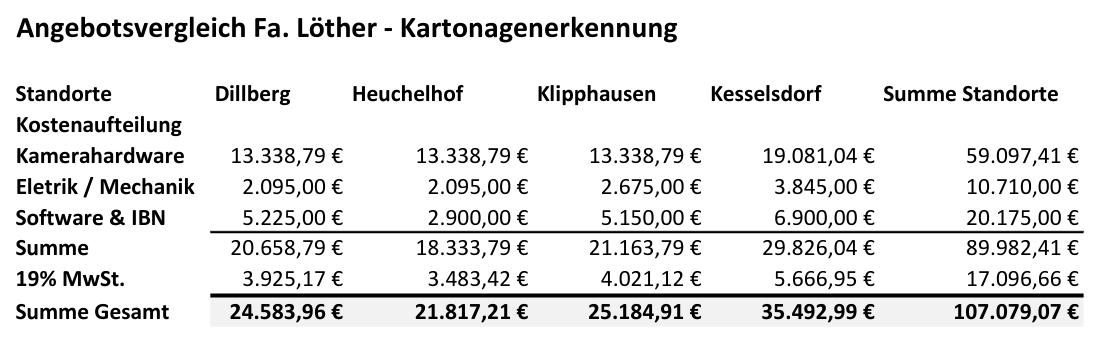
\includegraphics[width=1\textwidth]{pics/AngebotLoether.png}
  \end{figure}
\end{frame}


\begin{frame}[fragile]{Kostenverteilung Hardware}
  \begin{table}[htbp]
    \centering
    \begin{tabular}{lr}
      \textbf{Hardware}           & \textbf{Gesamt}         \\ \hline
      ARCELI Shield Board Kit     & \SI{17.99}{€}           \\
      AZDelivery 5 x Mega 2560 R3 & \SI{14.99}{€}           \\
      Benewake TF MINI PLUS       & \SI{182.40}{€}          \\
      Microsoft Lifecam Studio    & \SI{42.99}{€}           \\
      item-Systemprofile          & \SI{29.52}{€}           \\
      item-Verbindungsstücke      & \SI{192.00}{€}          \\
      item-Füße                   & \SI{48.00}{€}           \\
      Dell Wyse 5070 Thin Client  & \SI{450.00}{€}          \\
      \hline
      \textbf{Gesamtkosten}       & \textbf{\SI{977.89}{€}}
    \end{tabular}
  \end{table}
\end{frame}


\begin{frame}[fragile]{Kostenverteilung Personal und Hardware}
  \begin{table}[htbp]
    \centering
    \begin{tabular}{lrrr}
      \textbf{Personal}     & \textbf{Zeit in Stunden} & \textbf{Kosten pro Stunde}     & \textbf{Gesamt}          \\ \hline
      Auszubildender        & 80                       & \SI{6.00}{€} + \SI{15.00}{€}   & \SI{1680.00}{€}          \\
      Teamleitung           & 2                        & \SI{31.50}{€}  + \SI{15.00}{€} & \SI{93.00}{€}            \\
      Teammitglied          & 2                        & \SI{21.50}{€}  + \SI{15.00}{€} & \SI{73.00}{€}            \\
      Haustechnik           & 8                        & \SI{19.00}{€}  + \SI{15.00}{€} & \SI{272.00}{€}           \\ \hline
      \textbf{Gesamtkosten} &                          &                                & \textbf{\SI{2118.00}{€}}
    \end{tabular}
  \end{table}

  \vspace{0.4cm}

  \textbf{Gesamtkosten Personal und Hardware: \SI{3095.89}{€}}
\end{frame}



\section{Entwurf}
\begin{frame}[fragile]{Sensorträger}
  \begin{figure}[htpb]
    \centering
    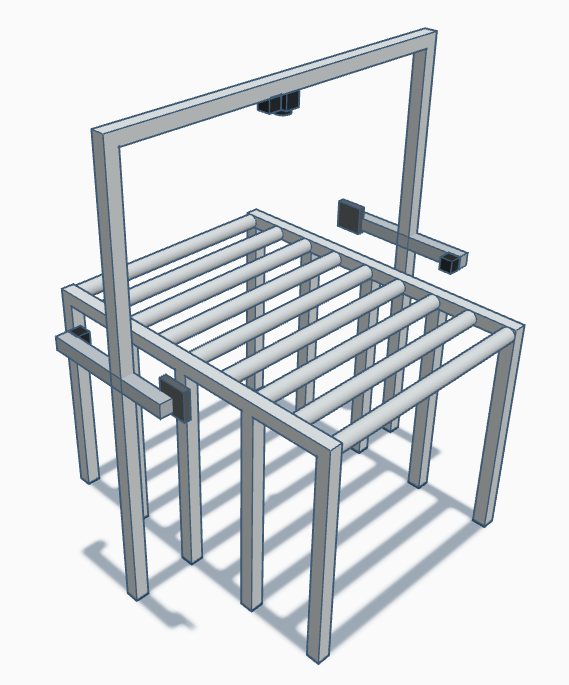
\includegraphics[width=0.6\textwidth]{files/Sensortraeger/Skizze_Sensor_Traeger_3D_verdreht_cropped.png}
  \end{figure}
\end{frame}


\begin{frame}[fragile]{Standort}
  \begin{figure}[htpb]
    \centering
    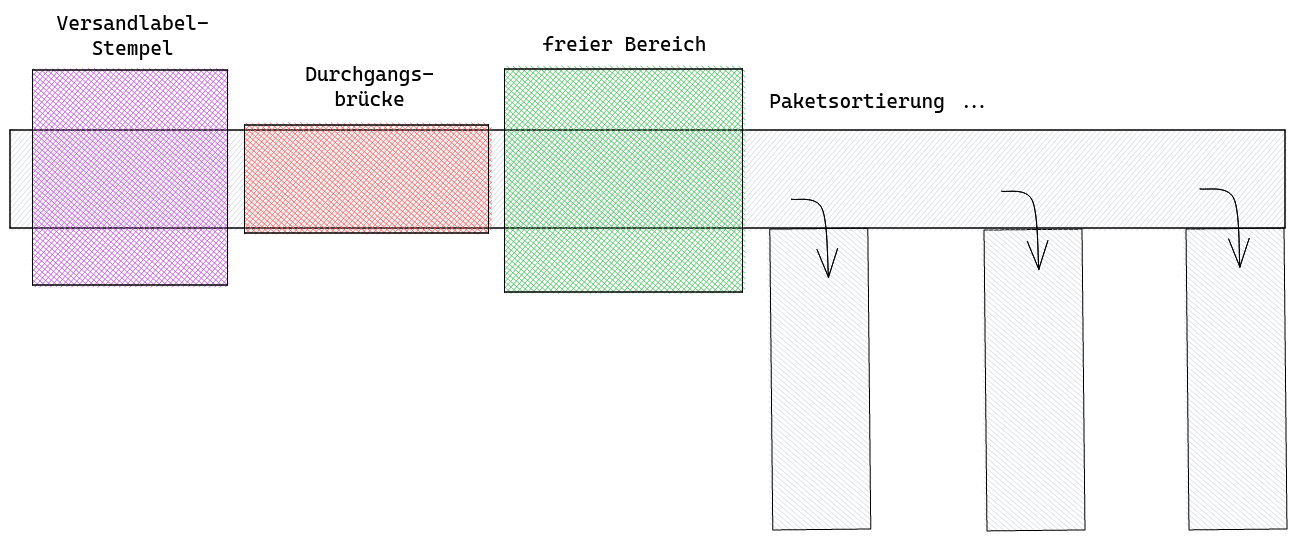
\includegraphics[width=1\textwidth]{pics/Versandanlage.png}
  \end{figure}
\end{frame}


\begin{frame}[fragile]{Programmübersicht}
  \begin{figure}[htpb]
    \centering
    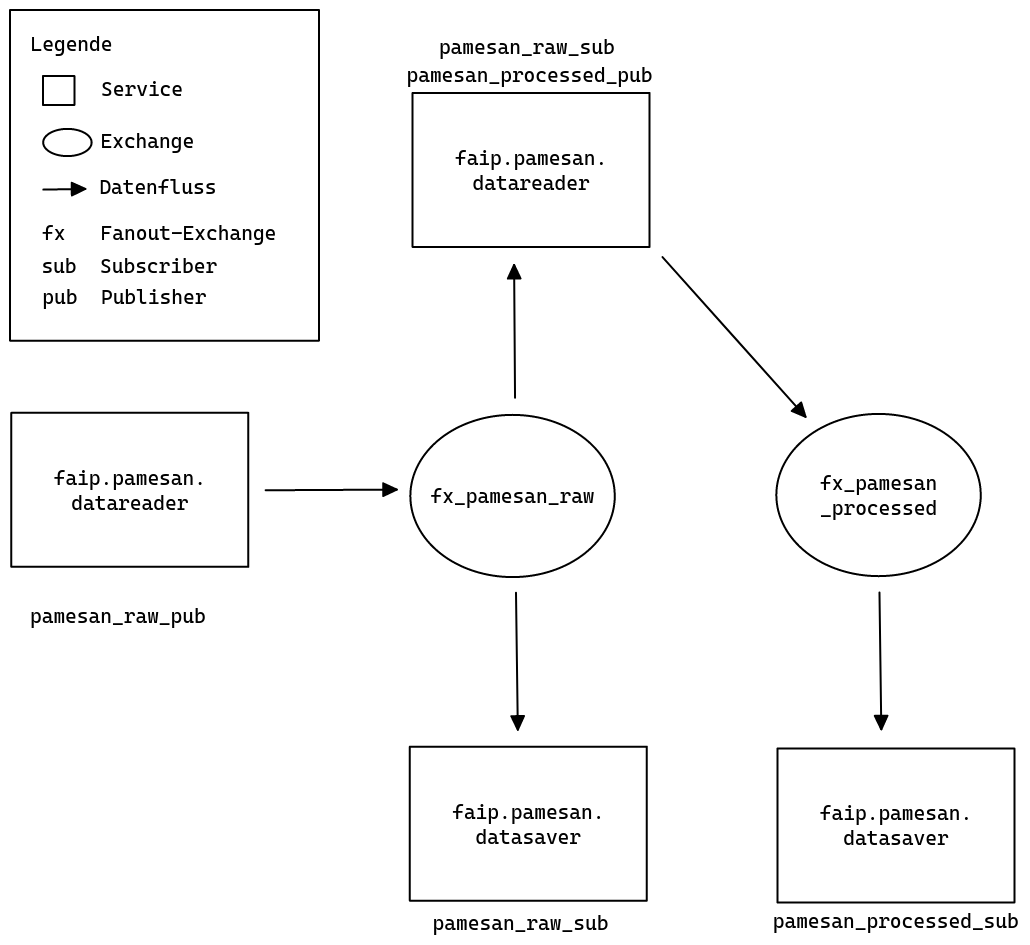
\includegraphics[width=0.75\textwidth]{pics/Architektur.png}
  \end{figure}
\end{frame}


\begin{frame}[fragile]{Datenmodell}
  \begin{figure}[htpb]
    \centering
    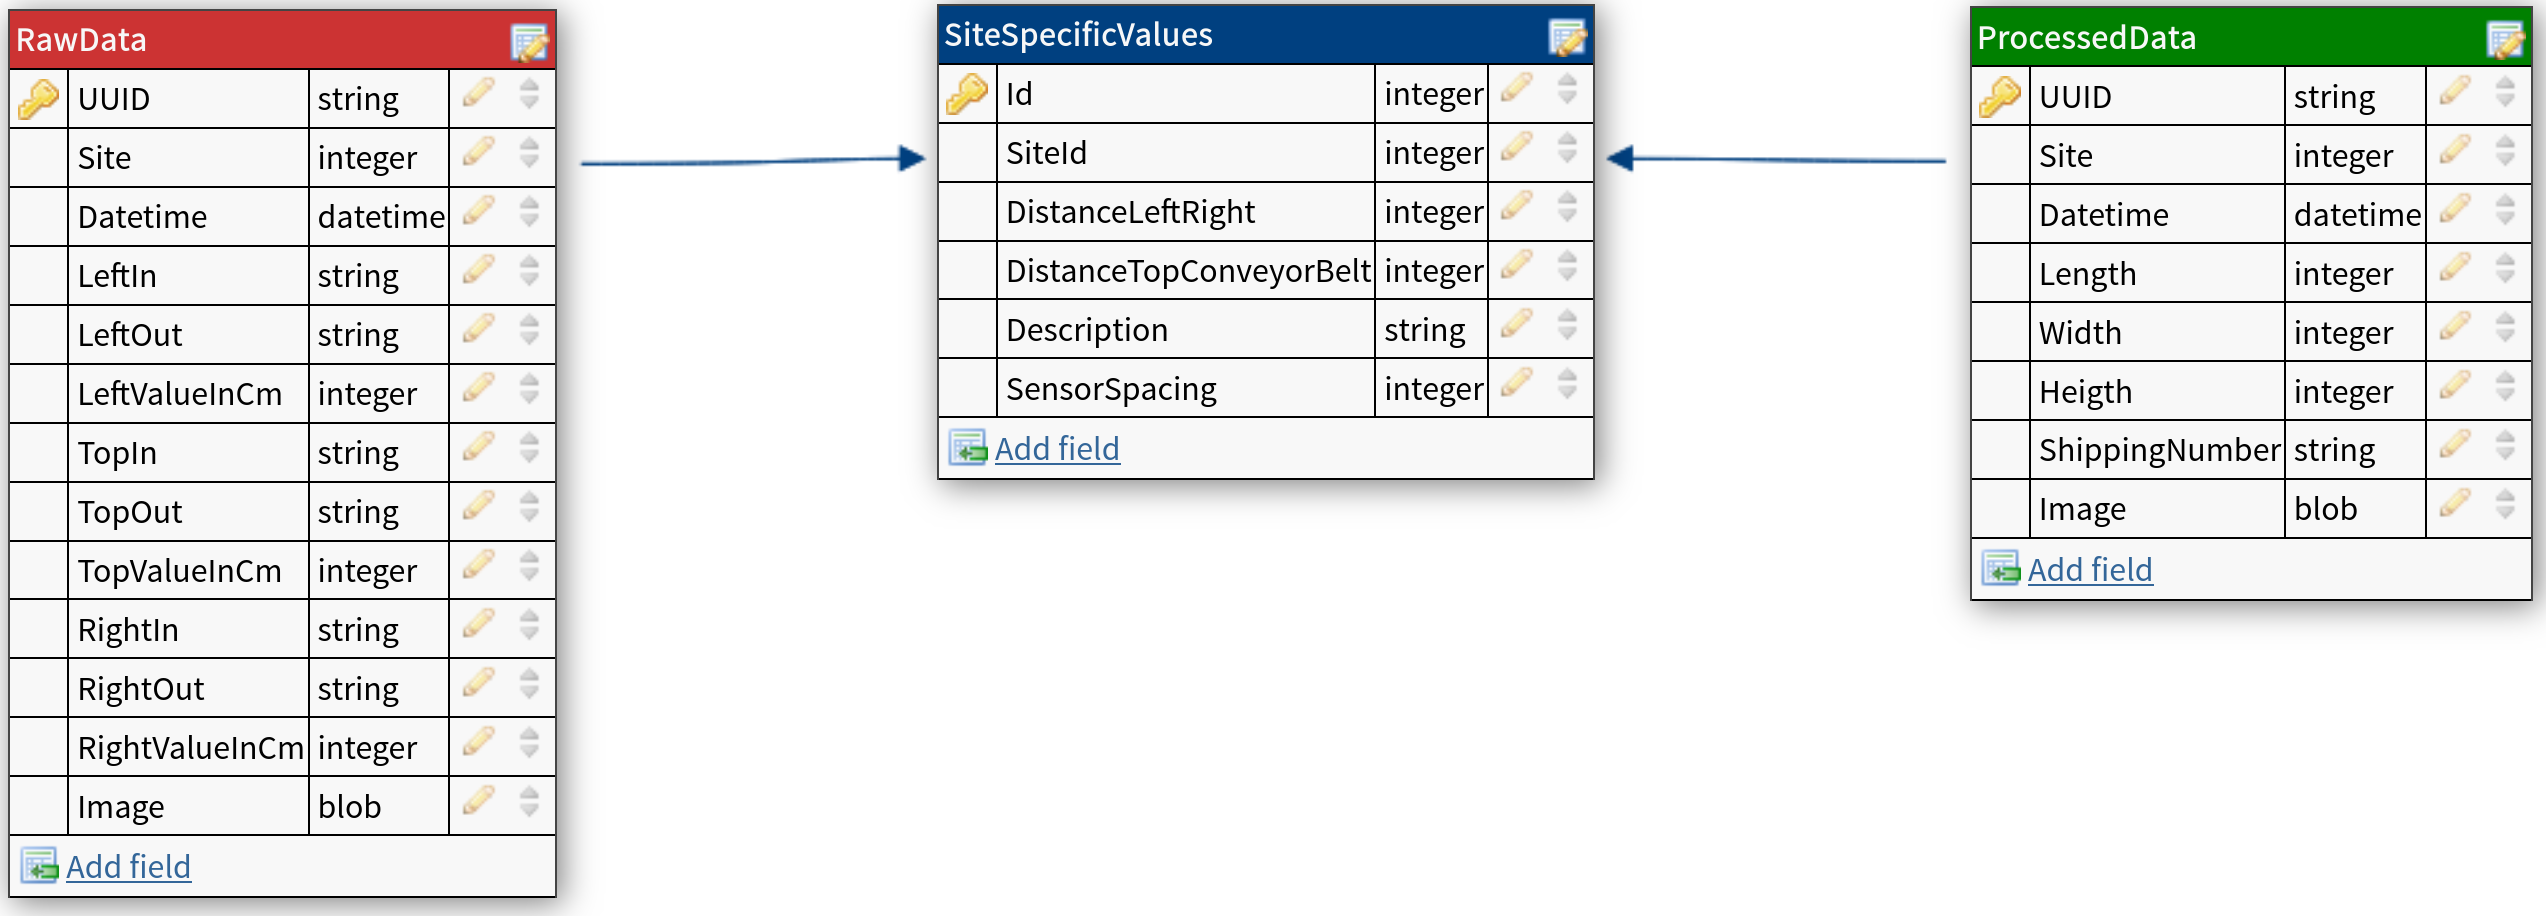
\includegraphics[width=1\textwidth]{pics/Tabellenmodell_schoen.png}
  \end{figure}
\end{frame}



\section{Implementierung}
\begin{frame}[fragile]{Lasersensor und Arduino}
  \begin{minipage}[t]{0.49\textwidth}
    \begin{figure}
      \centering
      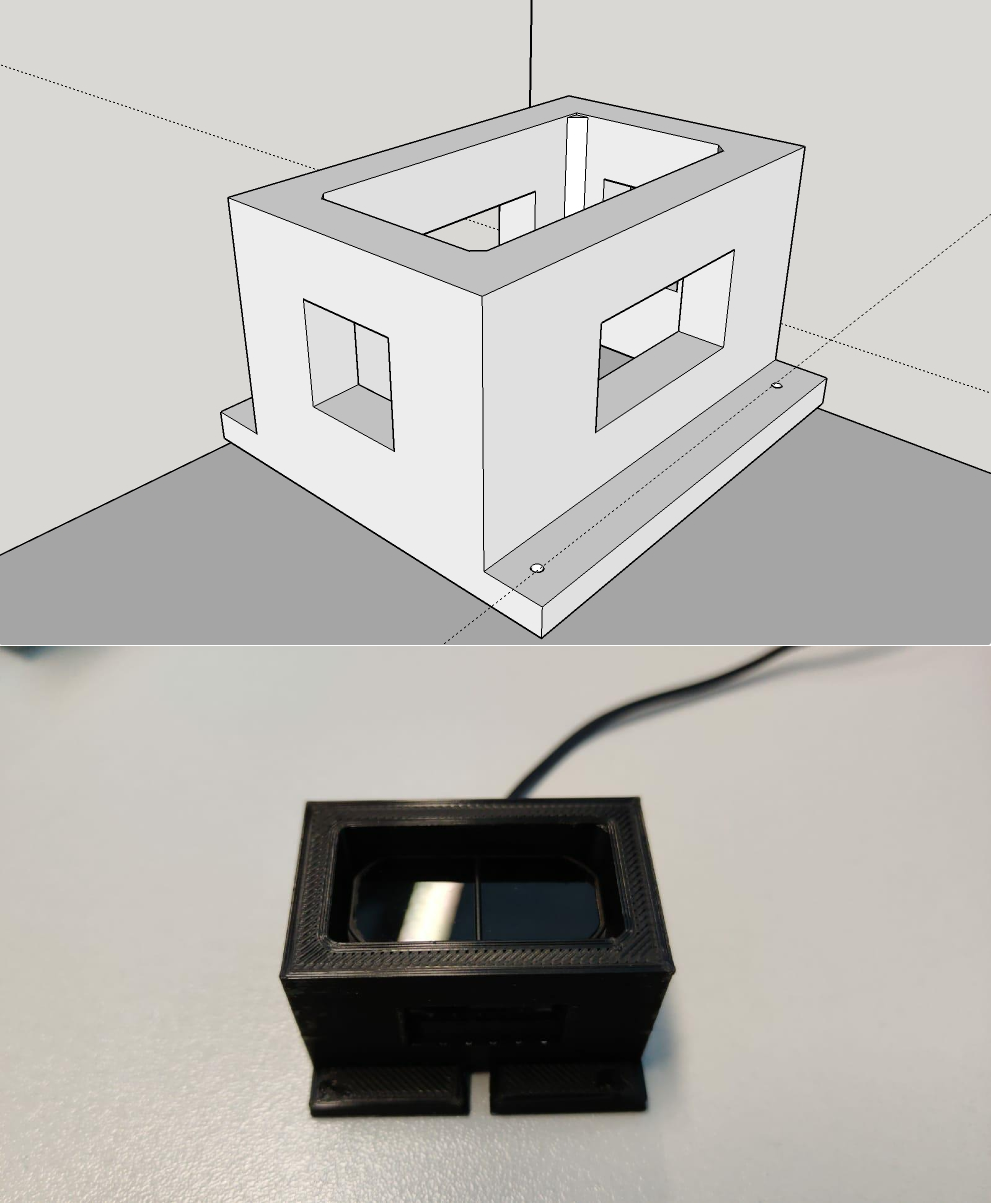
\includegraphics[width=1\textwidth]{pics/thingiverse_3D.png}
    \end{figure}
  \end{minipage}
  \begin{minipage}[t]{0.49\textwidth}
    \begin{figure}
      \centering
      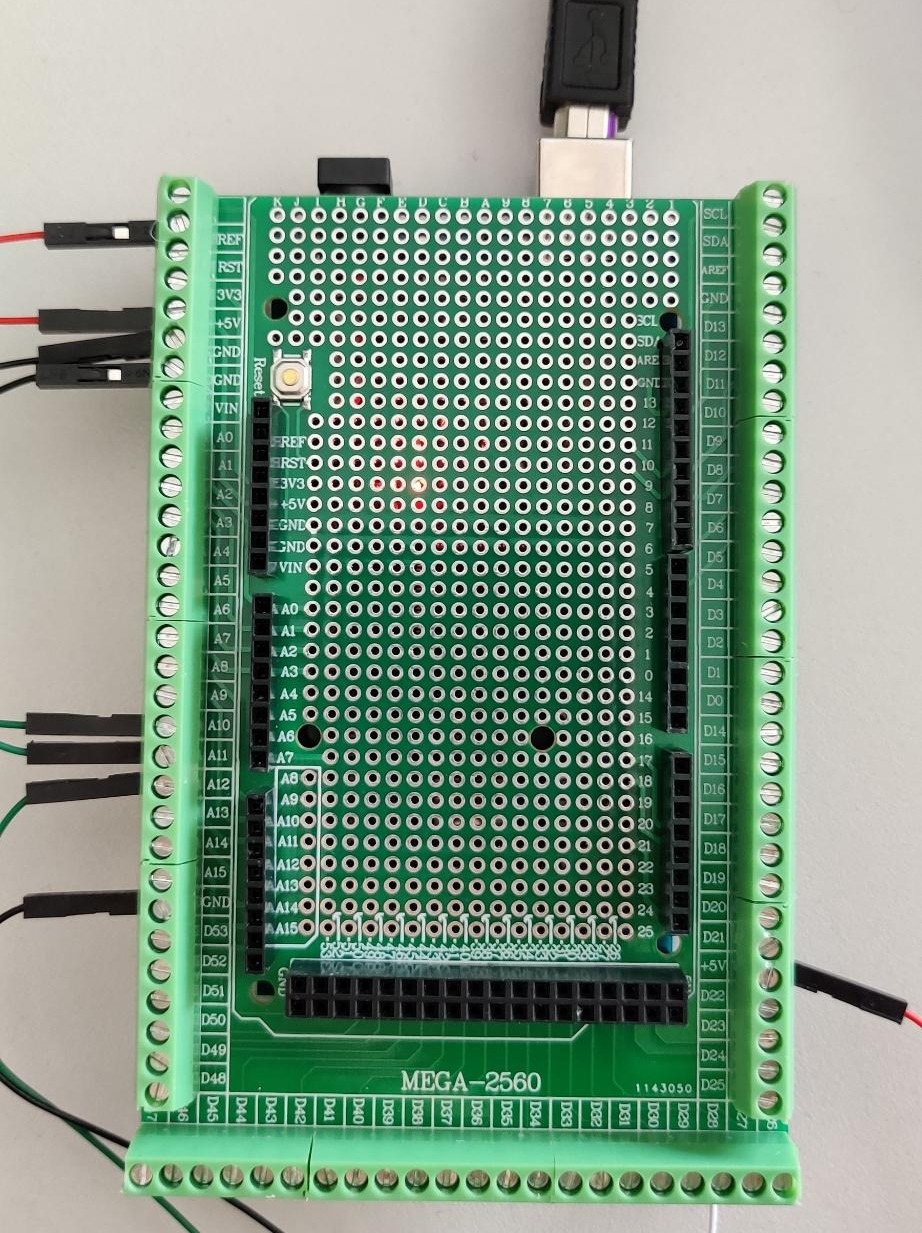
\includegraphics[width=1\textwidth]{pics/Arduino.jpeg}
    \end{figure}
  \end{minipage}
\end{frame}


\begin{frame}[fragile]{Umsetzung des Sensorträgers}
  \begin{figure}[htpb]
    \centering
    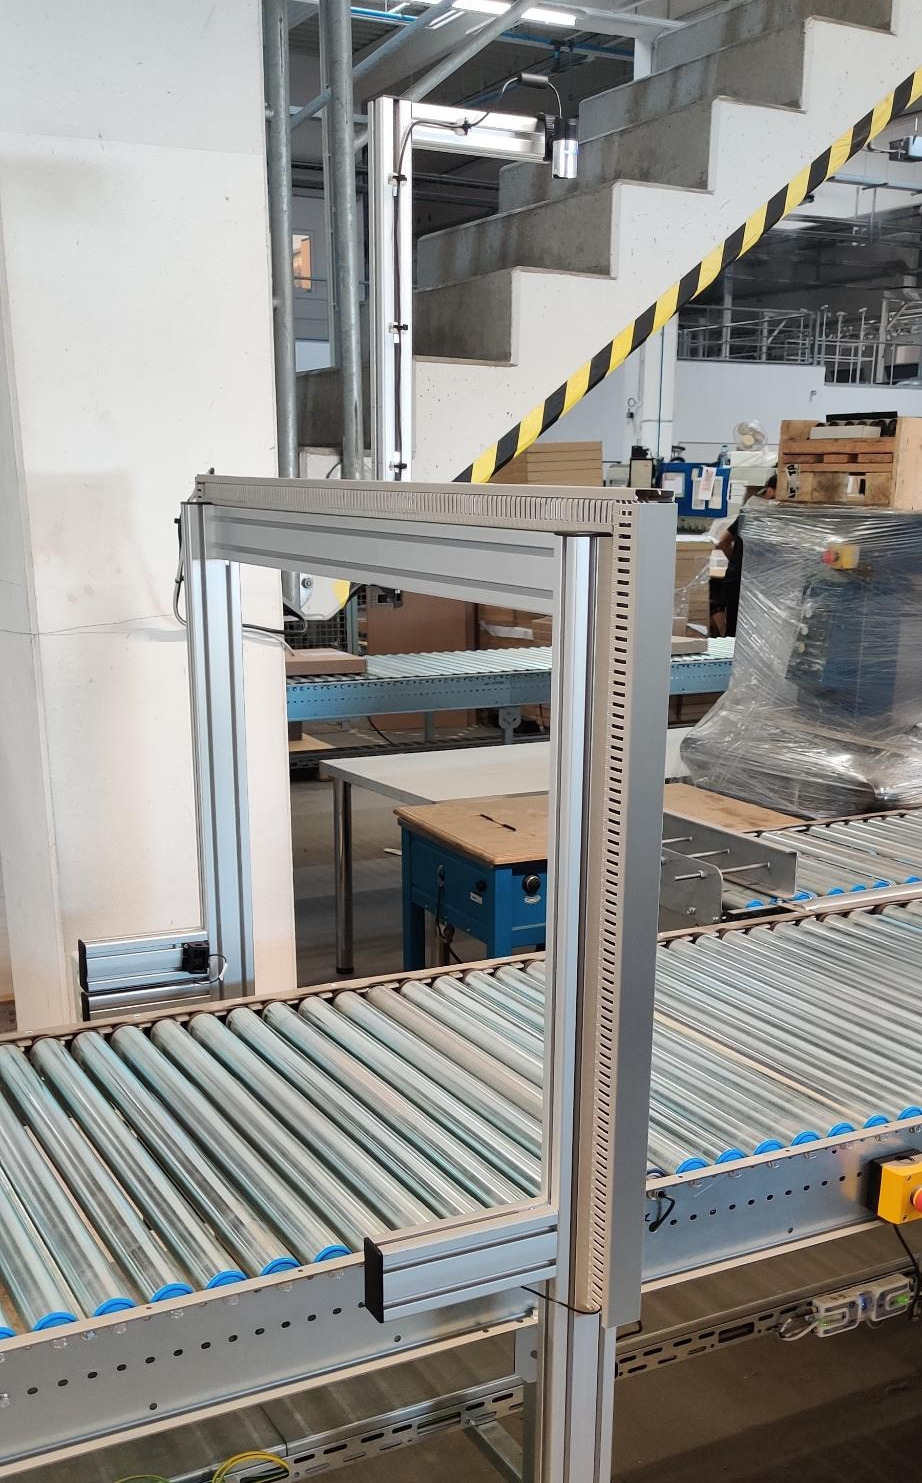
\includegraphics[width=0.45\textwidth]{pics/Sensortraeger_cropped.jpeg}
  \end{figure}
\end{frame}


\begin{frame}[fragile]{Implementierung des Ausleseservice}
  \begin{figure}[htpb]
    \centering
    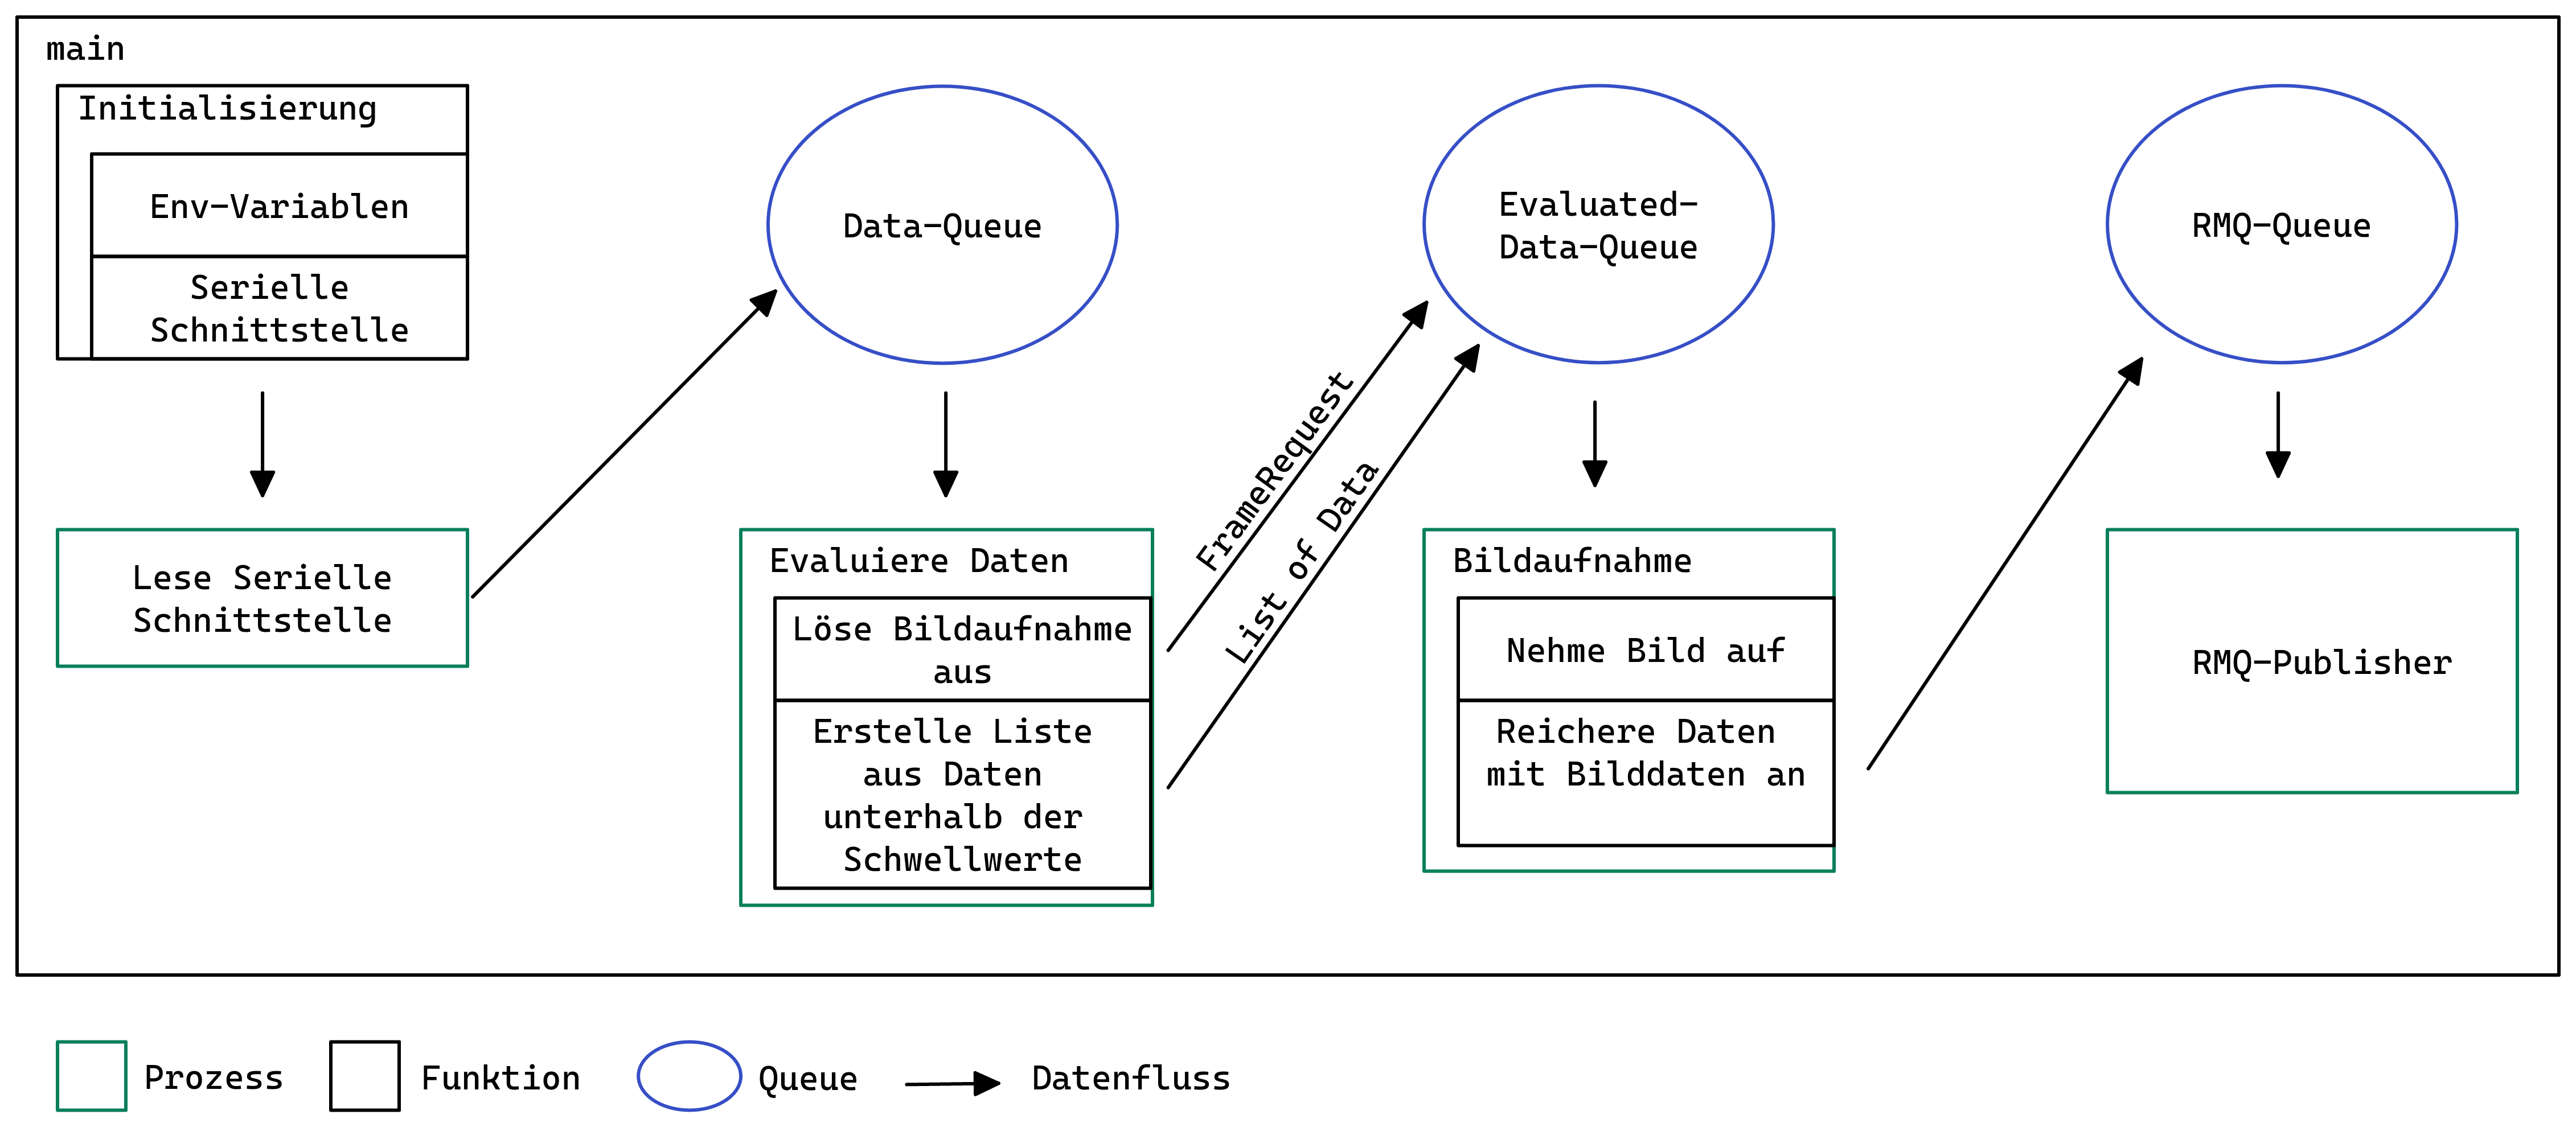
\includegraphics[width=1\textwidth]{pics/DataReaderDataFlow.png}
  \end{figure}
\end{frame}


\begin{frame}[fragile]{Implementierung des Ausleseservice -- Pika}
  \begin{lstlisting}[style=MyPythonStyle,
    breaklines=true, firstnumber=75]
def rmq_sender(queue: Queue):
  config_reader = EnvConfig()
  config_reader.initialize_env()
  pub = Publisher(config_reader)
  pub.connect()
  site_id = config_reader.get_site_id()
  while True:
      try:
          if not queue.empty():
              data = queue.get()
              hyd_data = data_hydration(data, site_id)
              pub.publish(hyd_data)

          time.sleep(0.5)
      except Exception as ex: <@\\\large\vdots@>
\end{lstlisting}
\end{frame}


\begin{frame}[fragile]{RabbitMQ}
  \alt<2>{
    \begin{figure}[htpb]
      \centering
      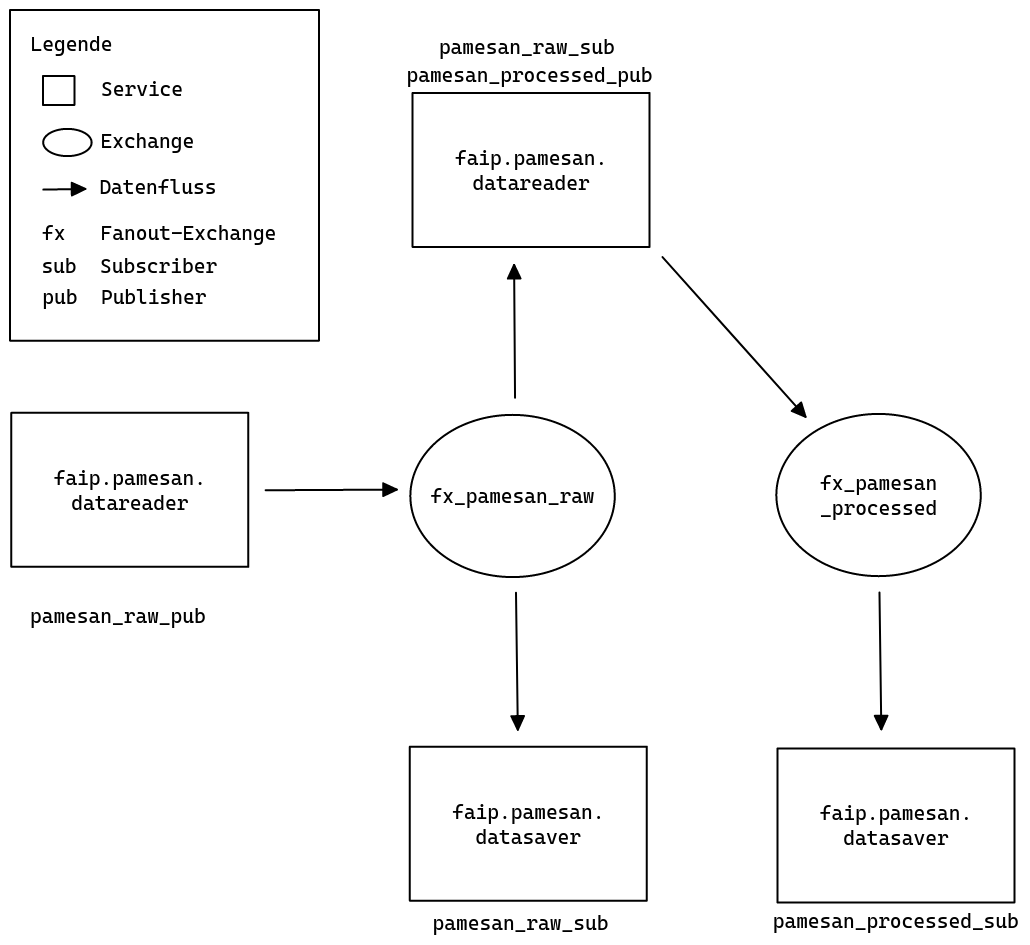
\includegraphics[width=0.75\textwidth]{pics/Architektur.png}
    \end{figure}}
  {\begin{figure}[htpb]
      \centering
      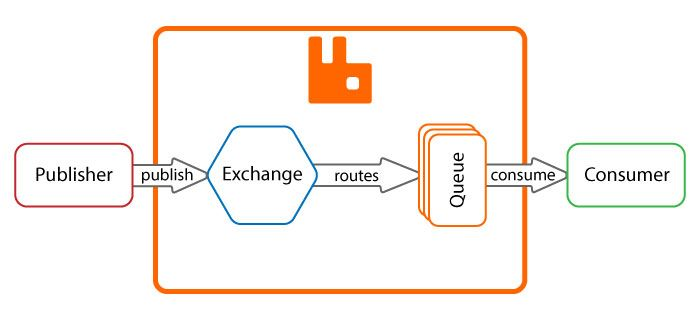
\includegraphics[width=1\textwidth]{pics/rabbitmq-broker.jpg}
    \end{figure}}
\end{frame}


\begin{frame}[fragile]{Implementierung der Datenbanktabellen}
  \begin{lstlisting}[style=sql-style,
    breaklines=true]
    CREATE TABLE PAMESAN.dbo.RawData (
        UUID uniqueidentifier NOT NULL,
        Site int NOT NULL,
        [Datetime] datetime NULL,
        LeftIn nvarchar(50) COLLATE Latin1_General_CI_AS NULL, <@\\\large\vdots \setcounter{lstnumber}{13}@>
        [Image] varbinary(MAX) NULL,
        CONSTRAINT PK_RawData PRIMARY KEY (UUID),
        CONSTRAINT RawData_FK FOREIGN KEY (Site) REFERENCES PAMESAN.dbo.SiteSpecificValues(Id)
    );
\end{lstlisting}
\end{frame}


\begin{frame}[fragile]{Implementierung des Datenspeicherservice}
  \smartdiagramset{
    uniform color list=white for 4 items,
    uniform arrow color=true,
    arrow color=gray!50!black,
    back arrow disabled=true}
  \smartdiagram[flow diagram:horizontal]{Commit auf main-branch,
    GitLab Pipeline, Docker Image, Docker Swarm}

  \pause

  \begin{lstlisting}[style=bash-style,
    breaklines=true]
    Scaffold-DbContext "Data Source=sql-mar-01.druckhaus.local; Initial Catalog=PAMESAN; persist security info=True; user id=pamesan-rw; password=******" Microsoft.EntityFrameworkCore.SqlServer -OutputDir DatabaseContext -Tables RawData, ProcessedData
\end{lstlisting}
\end{frame}


\begin{frame}[fragile]{Implementierung des Datenspeicherservice}
  \begin{lstlisting}[style=cSharpStyle,
    breaklines=true, firstnumber=38]
internal static void SaveDataToRaw(string data, PAMESANContext dbContext) {
  try {
    RawData rawData = JsonConvert.DeserializeObject<RawData>(data)!;

    dbContext.RawData.Add(rawData);
    dbContext.SaveChanges();
  }
  catch {
      throw;
  }
}
\end{lstlisting}
\end{frame}


\begin{frame}[fragile]{Implementierung des Datenverarbeitungsservice}
  \vspace{0.7cm}
  \begin{minipage}[c][8cm]{\textwidth}
    \centering
    \smartdiagramset{
      uniform color list=white for 5 items,
      circular final arrow disabled=true,
      circular distance=2.25cm,
      arrow tip=to,
      arrow line width=2pt,
      uniform arrow color=true,
      arrow color=gray!50!black,
      additions={
          additional item bottom color=white,
          additional item border color=gray,
          additional item shadow=drop shadow,
          additional item offset=0.65cm,
          additional arrow line width=2pt,
          additional arrow tip=to,
          additional arrow color=gray!50!black,
        }
    }
    \smartdiagramadd[circular diagram]{
      Paketerkennung,Zuschnitt,Labelerkennung,Barcode auslesen,Paketgröße berechnen
    }{
      above of module1/RMQ-Subscriber,right of module5/RMQ-Publisher
    }
    \smartdiagramconnect{to-}{module1/additional-module1}
    \smartdiagramconnect{-to}{module5/additional-module2}
  \end{minipage}
\end{frame}


\begin{frame}[fragile]{Labeln der Bilder}
  \begin{figure}[htpb]
    \centering
    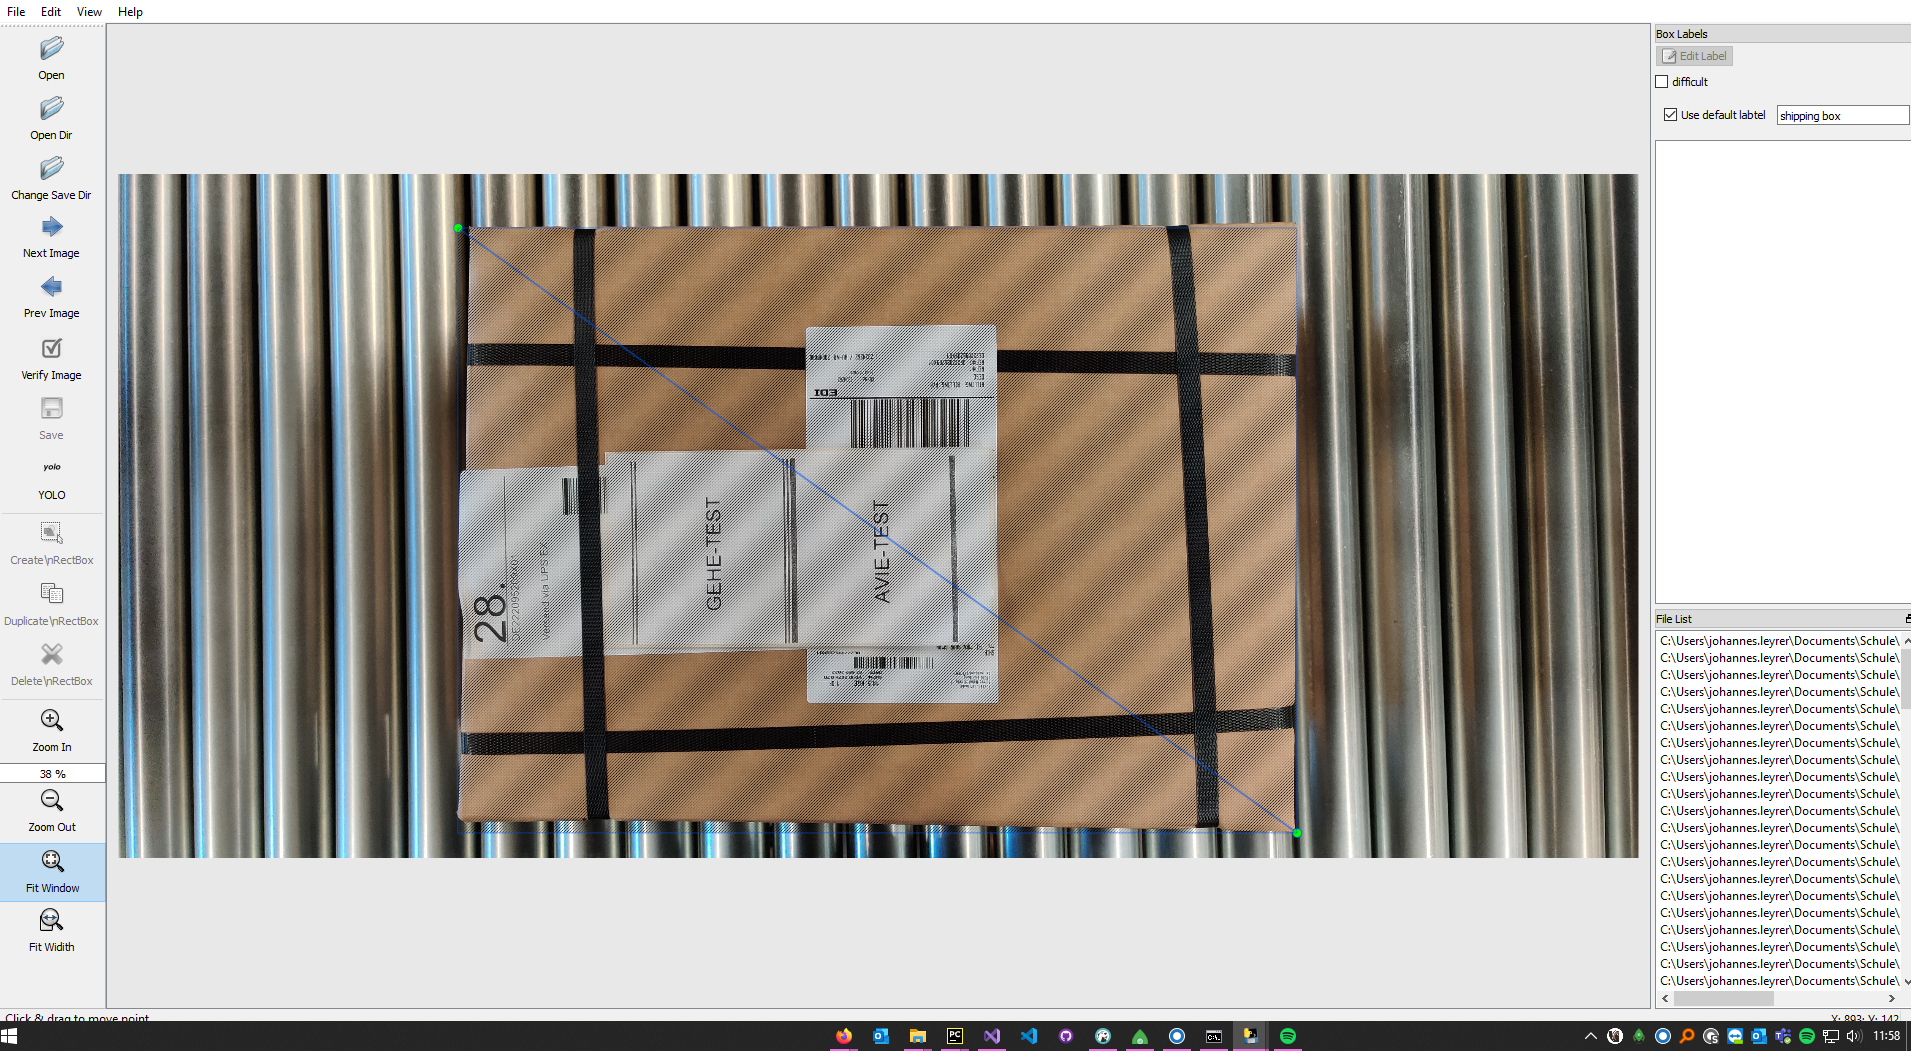
\includegraphics[width=1\textwidth]{pics/labelImg.png}
  \end{figure}
\end{frame}


\begin{frame}[fragile]{Training des YOLOv7-Models}
  \begin{lstlisting}[style=bash-style,
    breaklines=true]
    python train.py --device 0 --batch-size 16 --epochs 100 --img 640 640 --data data/custom_data.yaml --hyp data/hyp.scratch.custom.yaml --cfg cfg/training/yolov7_custom.yaml --weights yolov7.pt --name yolo7-custom
  \end{lstlisting}
\end{frame}


\begin{frame}[fragile]{Ergebnis des YOLOv7-Models}
  \begin{figure}[htpb]
    \centering
    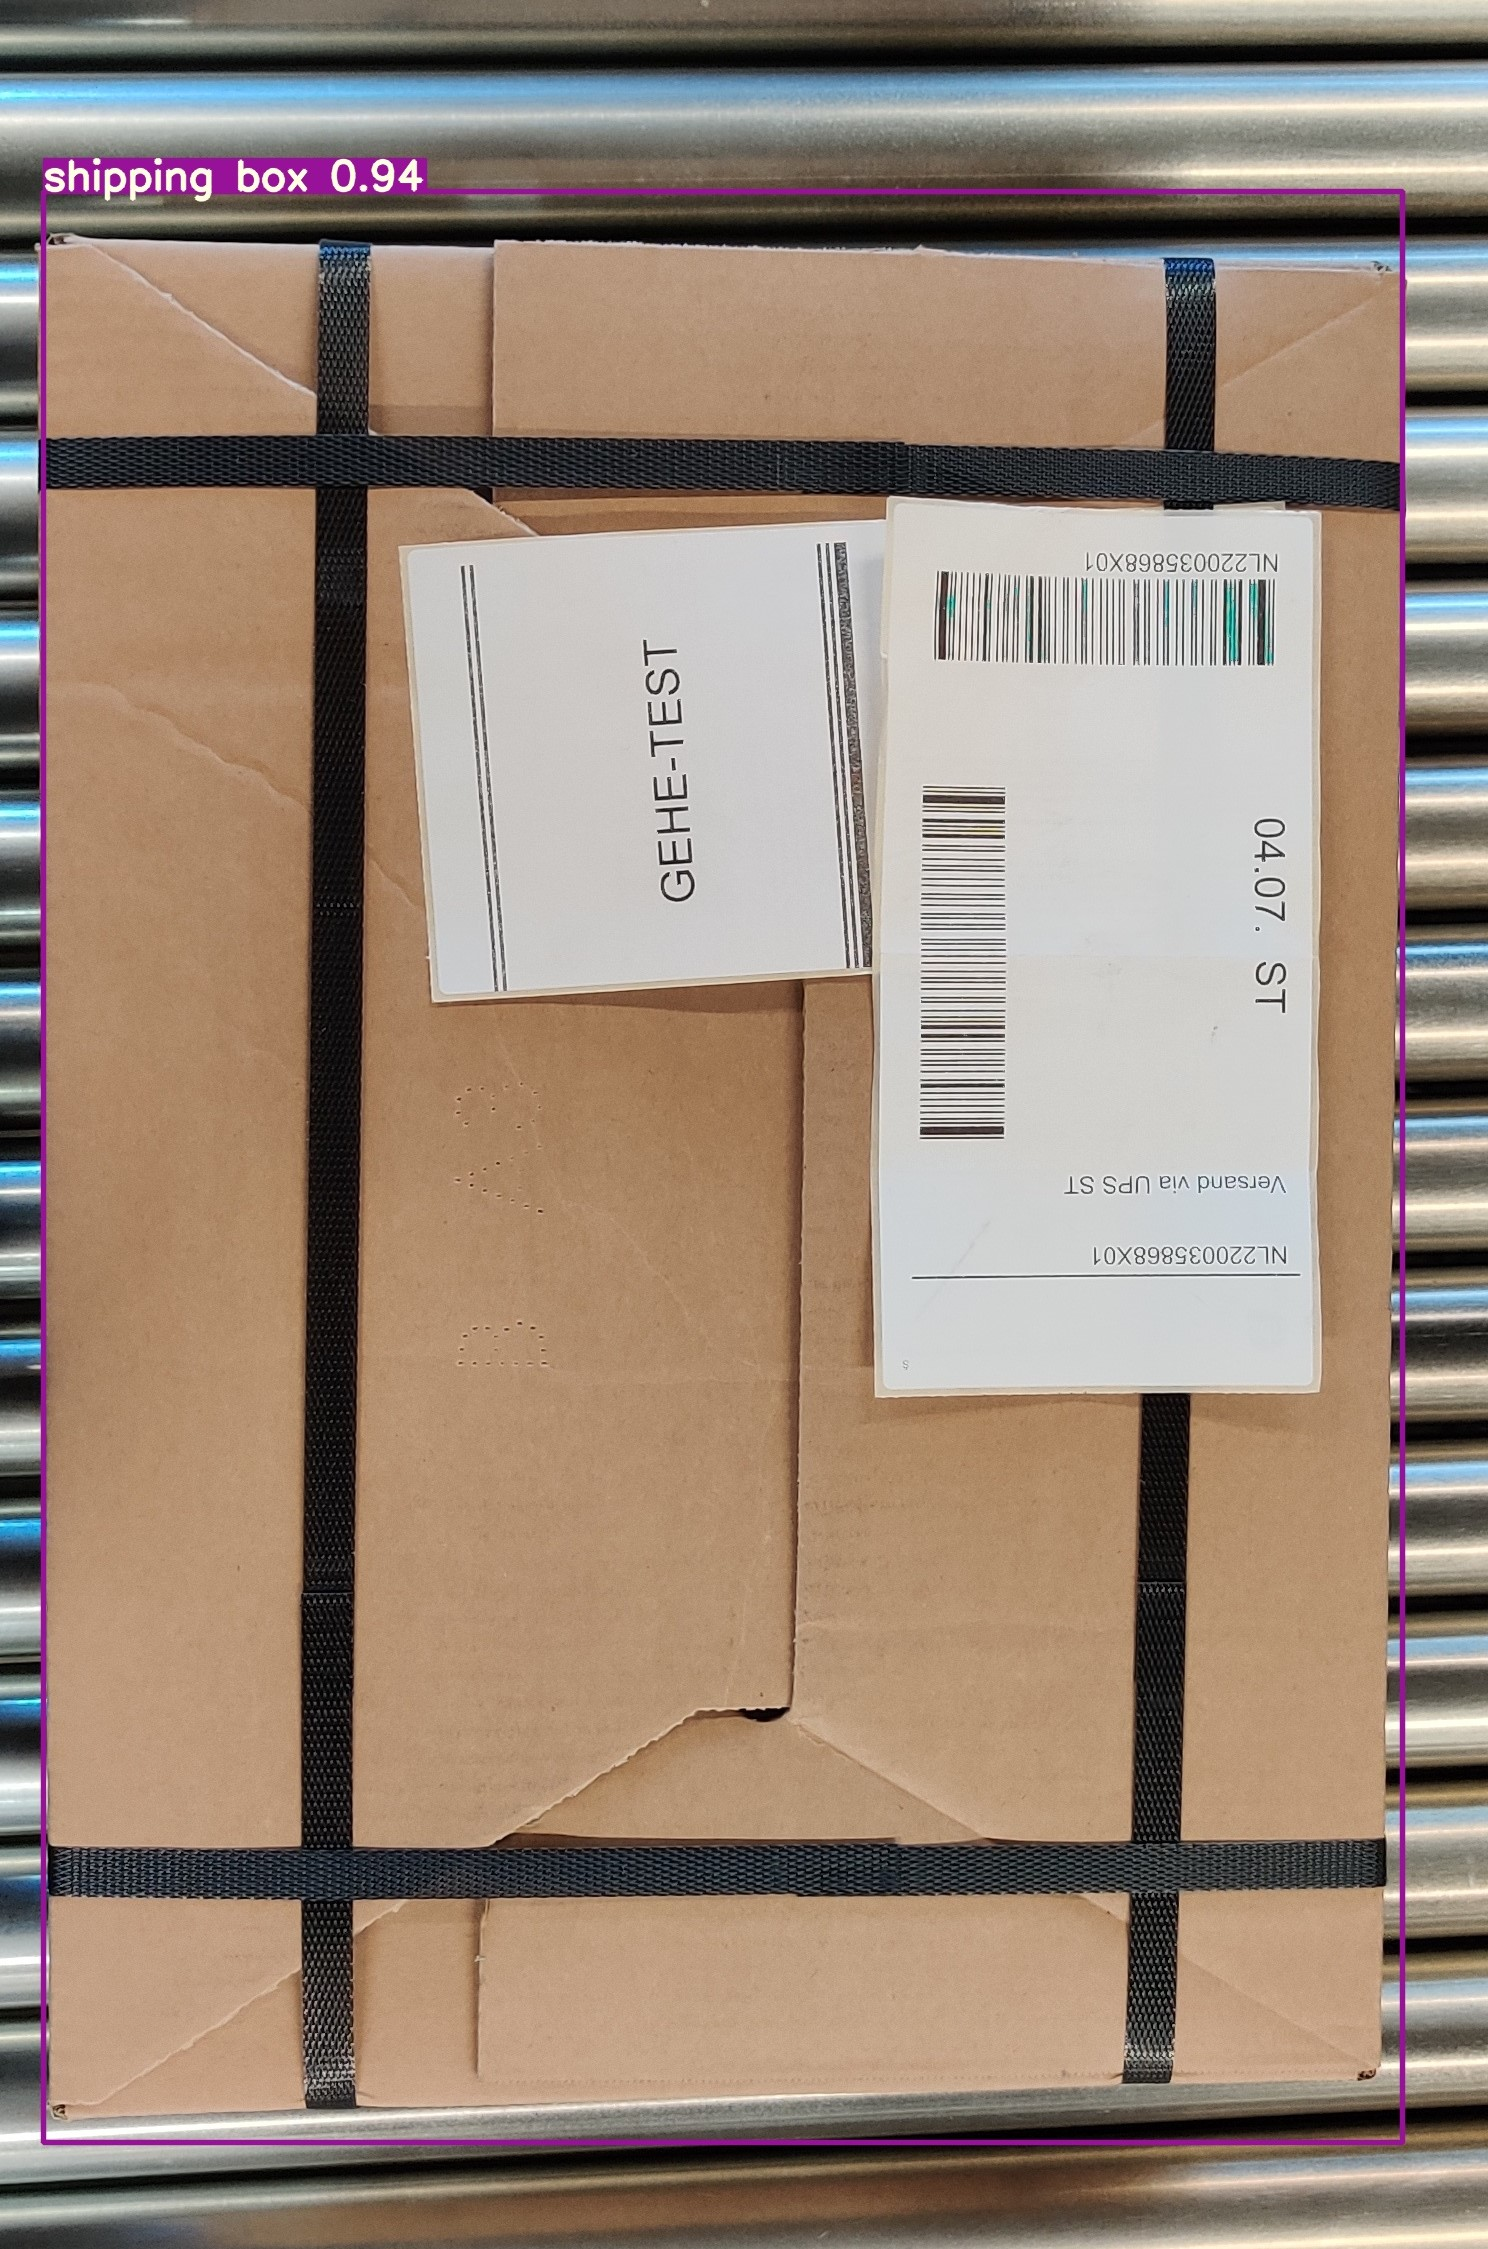
\includegraphics[angle=90,origin=c,width=1\textwidth]{pics/detectShippingBox.jpg}
  \end{figure}
\end{frame}


\begin{frame}[fragile]{Auslesen des Versandlabels}
  \begin{figure}[htpb]
    \centering
    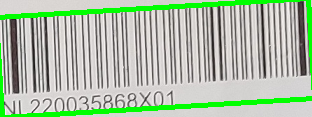
\includegraphics[width=1\textwidth]{pics/barcode.png}
  \end{figure}
\end{frame}


\begin{frame}[fragile]{Berechnung der Paketgröße}
  \textbf{HIER BERECHNUNG ERSTELLEN UND EINFÜGEN}
\end{frame}



\section{Fazit}
\begin{frame}[fragile]{Soll-/Ist-Vergleich}
  \begin{tikzpicture}

    \draw (0cm,0cm) -- (9.5cm,0cm);  %Abzisse
    \draw (0cm,0cm) -- (0cm,-0.1cm);  %linkes Ende der Abzisse
    \draw (9.5cm,0cm) -- (9.5cm,-0.1cm);  %rechtes Ende der Abzisse

    \draw (-0.1cm,0cm) -- (-0.1cm,5cm);  %Ordinate
    \draw (-0.1cm,0cm) -- (-0.2cm,0cm);  %unteres Ende der Ordinate
    \draw (-0.1cm,5cm) -- (-0.2cm,5cm) node [left] {h};  %oberes Ende der Ordinate

    \foreach \x in {10,20,...,40}  %Hilfslinien
    \draw[gray!50, text=black] (-0.2 cm,\x * 0.1 cm) -- (9.5 cm,\x * 0.1 cm)
    node at (-0.5 cm,\x * 0.1 cm) {\x};  %Beschriftung der Hilfslinien

    \node at (4.5cm,5.5cm) {Abschließender Zeitablauf};  %Überschrift

    \foreach \x/\y/\country in {0.5/10/Analyse,  %\x ist Anfang der Säulen
        2/8/Entwurf,  %\y ist Höhe der Säulen
        3.5/39/Implementierung,
        5/5/Test,
        6.5/6/Einführung,
        8/12/Dokumentation}
      {
        \draw[fill=mSybilaRed] (\x cm,0cm) rectangle (0.5cm+\x cm,\y * 0.1 cm) %die Säulen
        node at (0.2cm + \x cm,\y * 0.1 cm + 0.3cm) {\y}; %die Prozente über den Säulen
        \node[rotate=45, left] at (0.6 cm +\x cm,-0.1cm) {\country}; %Säulenbeschriftung
      };

    \foreach \x/\y in {0.9/10,  %\x ist Anfang der Säulen
        2.4/8,  %\y ist Höhe der Säulen
        3.9/46,
        5.4/2,
        6.9/2,
        8.4/12}
      {
        \draw[fill=darkgreenshade] (\x cm,0cm) rectangle (0.5cm+\x cm,\y * 0.1 cm) %die Säulen
        node at (0.25cm + \x cm,\y * 0.1 cm + 0.3cm) {\y}; %die Prozente über den Säulen
      };

    \draw[fill=mSybilaRed] (7cm,4.5cm) rectangle (7.2cm,4.7cm) node at (8cm,4.6cm) {h geplant};
    \draw[fill=darkgreenshade] (7cm,4cm) rectangle (7.2cm,4.2cm) node at (8.2cm,4.1cm) {h gebraucht};

  \end{tikzpicture}
\end{frame}


\begin{frame}[fragile]{Lessons Learned und Ausblick}
  \textbf{Lessons Learned}
  \begin{itemize}
    \item YOLOv7 als mit geringem Vorwissen leicht einsetzbarer Objektdetektor
          \pause
    \item Pufferzeit sollte \SI{2}{\percent} der Gesamtzeit betragen
          \pause
    \item Industriekamera $>$ Webcam $\rightarrow$ KEYENCE-Scanner
  \end{itemize}

  \pause

  \textbf{Ausblick}
  \begin{itemize}
    \item Verwendung KEYENCE-Scanner und Umschreiben auf C\#
          \pause
    \item Verknüpfung erfasster Abmessungen mit bekannten Kartonagen
          \pause
    \item Aufbau an anderen Standorten
  \end{itemize}
\end{frame}




% Show the slide as if horizontal blinds were pulled away.
% \transblindshorizontal

% Show the slide as if vertical blinds were pulled away.
% \transblindsvertical

% Show the slide by moving to the center from all four sides.
% \transboxin

% Show the slide by showing more and more of a rectangular area that is centered on the slide center
% \transboxout

% Slowly dissolve what was shown before
% \transdissolve

% Glitter sweeps in specified direction
% \transglitter

% Show the slide by sweeping two vertical lines from the sides inward.
% \transsplitverticalin

% Show the slide by sweeping two vertical lines from the center outward.
% \transsplitverticalout

% Show the slide by sweeping two horizontal lines from the sides inward.
% \transsplithorizontalin

% Show the slide by sweeping two horizontal lines from the center outward.
% \transsplithorizontalout

% Sweeps single line in specified direction
% \transwipe

% Show slide specified number of seconds
% \transduration{2}

% Show the slide by pushing what was shown before off the screen using the new content.
% \transpush

% Replace the previous slide directly (default behaviour).
% \transreplace

% Show the slide by covering the content that was shown before
% \transcover




% \begin{frame}
%   \transglitter<2-4> %means that the effect is within the frame but only for slide 2 to 4

%   \frametitle{Test}
%   \begin{itemize}
%     \item \onslide<2->{One} %shown from slide 2 till last slide of this frame
%     \item \onslide<3->{Two}
%     \item \onslide<4->{Three}
%   \end{itemize}
% \end{frame}



% \section{CO$_2$-Grenzwerte für eine unbedenkliche Atemluft}
% \begin{frame}[fragile]{CO$_2$-Grenzwerte für eine unbedenkliche Atemluft}
%   \begin{itemize}
%     \item Atmosphäre hat 400 ppm CO$_2$ \autocite{umweltbundesamt}
%     \item ab 1000 ppm CO$_2$ bedenklich laut DGUV ASR A3.6 \autocite{ASR}
%     \item ab 950 ppm CO$_2$ bedenklich laut DIN EN 16798-1 \autocite{din_en_16798}
%   \end{itemize}
% \end{frame}

% \begin{frame}[fragile]{CO$_2$-Grenzwerte für eine unbedenkliche Atemluft}
%   \begin{table}
%     \caption{nach DGUV ASR A3.6 \autocite{ASR}}
%     \begin{tabular}{ |c|p{0.49\textwidth}|}
%       \hline
%       CO$_2$-Konzentration in ppm & Bewertung               \\ \hline
%       $<$1000                     & hygienisch unbedenklich \\ \hline
%       1000-2000                   & hygienisch auffällig    \\ \hline
%       $>$2000                     & hygienisch inakzeptabel \\ \hline
%     \end{tabular}
%   \end{table}
%   \begin{table}
%     \caption{nach DIN EN 16798-1 \autocite{din_en_16798}}
%     \begin{tabular}{|c|p{0.49\textwidth}|}
%       \hline
%       CO$_2$-Konzentration in ppm & Bewertung                 \\ \hline
%       $<$950                      & Hohe Raumluftqualität     \\ \hline
%       950-1200                    & Mittlere Raumluftqualität \\ \hline
%       1200-1750                   & Mäßige Raumluftqualität   \\ \hline
%       $>$1750                     & Niedrige Raumluftqualität \\ \hline
%     \end{tabular}
%   \end{table}
% \end{frame}

% \section{Auswirkungen eines zu hohen CO$_2$-Gehaltes in der Raumluft}
% \begin{frame}[fragile]{Auswirkungen eines zu hohen CO$_2$-Gehaltes in der Raumluft}
%   \begin{itemize}
%     \item verringerte Konzentrationsfähigkeit
%     \item verringerte Leistungsfähigkeit
%     \item Halsschmerzen
%     \item Kopfschmerzen
%     \item Unwohlsein
%     \item Müdigkeit
%     \item Hustenanfälle
%   \end{itemize}

%   Quellen: \autocite{umweltbundesamt} \autocite{din_en_16798} \autocite{ASR} \autocite{kajtar} \autocite{zhang} \autocite{myhrvold} \autocite{tiesler}
% \end{frame}

% \section{Hardwaretechnische Umsetzung}

% \begin{frame}[fragile]{Raspberry Pi 3B+}
%   \begin{figure}
%     \centering
%     \captionsetup{justification=centering}
%     \includegraphics[width=0.55\textwidth]{pictures/RasPi.png}
%     \caption{Raspberry Pi 3B+ \autocite{rasPi}}
%   \end{figure}
% \end{frame}

% \begin{frame}[fragile]{CO$_2$-Sensor}
%   \begin{figure}
%     \centering
%     \captionsetup{justification=centering}
%     \includegraphics[trim={0 10cm 0 10cm},clip,width=0.85\textwidth]{pictures/co2monitor.png}
%     \caption{TFA Dostmann AIRCO2NTROL MINI \autocite{co2monitor}}
%   \end{figure}
% \end{frame}


% \section{Softwaretechnische Umsetzung}

% \subsection{Grundlagen}
% \begin{frame}[fragile]{Grundlagen}
%   \begin{minipage}[t]{0.49\textwidth}
%     \begin{itemize}
%       \item Linux-Distribution inklusive mitgelieferter Standardsoftware
%       \item Docker
%       \item Python
%       \item FastAPI
%       \item React
%       \item ChartJs
%       \item SQLite
%     \end{itemize}
%   \end{minipage}
%   \begin{minipage}[t]{0.49\textwidth}
%     \begin{figure}
%       \centering
%       \captionsetup{justification=centering}
%       \includegraphics[width=1\textwidth]{pictures/SoftwareKomponenten.png}
%       \caption{Verwendete Softwarekomponenten \autocite{dockerLogo}\autocite{fastapiLogo}\autocite{sqliteLogo}\autocite{reactLogo}\autocite{pythonLogo}\autocite{chartjsLogo}}
%     \end{figure}
%   \end{minipage}
% \end{frame}

% \subsection{Zusammenspiel der Softwarekomponenten}

% \begin{frame}[fragile]{Zusammenspiel der Softwarekomponenten}
%   \begin{figure}
%     \centering
%     \captionsetup{justification=centering}
%     \includegraphics[width=0.6\textwidth]{pictures/SoftwareZusammenspiel.png}
%     \caption{Zusammenspiel der Softwarekomponenten \autocite{co2monitor}\autocite{rasPi}}
%   \end{figure}
% \end{frame}

% \subsection{Aufbau und Einrichtung der Softwarekomponenten}

% \begin{frame}[fragile]{Aufbau und Einrichtung der Softwarekomponenten}

%   \begin{minipage}[t]{0.49\textwidth}
%     \begin{itemize}
%       \item Backend: Python mit FastAPI
%       \item Frontend: React und ChartsJs
%       \item Lese-Software: Python-Script
%       \item Datenbank: SQLite
%     \end{itemize}
%   \end{minipage}

%   \begin{lstlisting}[language=Bash]
%     docker-compose -f docker-compose.yml up -d
%   \end{lstlisting}
% \end{frame}

% \section{Fazit}
% \begin{frame}[fragile]{Fazit}
%   \begin{minipage}[t]{0.80\textwidth}
%     \textbf{Ergebnisse:}\newline
%     \begin{itemize}
%       \item bestätigte Relevanz der Raumluftqualität
%       \item bestätigte Verbindung zwischen hohen CO$_2$-Konzentrationen und verminderter Konzentrationsfähigkeit/Produktivität
%       \item schaffen einer kostengünstigen Möglichkeit zur selbstständigen Kontrolle der Raumluftqualität
%     \end{itemize}
%   \end{minipage}
% \end{frame}

\begin{frame}[standout]
  Fragen?
\end{frame}

\appendix

\begin{frame}[allowframebreaks]{Literaturverzeichnis}

  \printbibliography[title={Quellenverzeichnis}]

\end{frame}

\begin{frame}[standout]
  Danke für die Aufmerksamkeit!
\end{frame}
\end{document}
